% In this section, we introduce a formal model of a distributed stream processing system. After that, we define the notions of delivery guarantees in a regular way.

\subsection{Motivation}
The concept of {\em consistency} is traditionally expressed in terms of the transactional behavior, known as the ACID properties of transactions in the databases. 
 These properties ensure that the (database) state is consistent to the degree required by the specified isolation level, providing consistency of processing. 
 However, database systems are not used standalone: they interact with client applications.
  From the client perspective,   the notion of consistency also includes {\em delivery guarantees} as well. {\em At-least-once} ensures that input data are not lost, {\em at-most-once} eliminates duplicate processing, and {\em exactly-once} combines both ensuring the absence of input data losses and repeated delivery of results. An implementation of exactly-once processing of transactions based on persistent queues is described in~\cite{DBLP:books/mk/WeikumV2002}.

Delivery guarantees are typically not considered in batch processing systems, because they always ensure atomicity between reading input data, processing, and delivery of results. In other words, it means that each record within a batch is processed exactly-once. This is achieved by consecutive processing of batches, persistent storage for all intermediate results, and reprocessing of all suspected failures. 
A disadvantage of this approach is the impossibility to deliver any results while the processing is not complete.

In contrast,   consistency guarantees for stream processing systems are commonly declared in terms of delivery only. 
A pitfall here is that terms like {\em exactly-once} and {\em at-least-once} hide the fact that system state must also be consistent with input and output in order to achieve correct results. 
In the absence of formal definitions, such terms can lead to an improper perception that the state does not play an essential role in consistency enforcement. 

The problem shows up if some streaming elements do not commutate within an operation in a data flow. 
Let us consider a data flow with an operation that concatenates input strings and delivers it after each item. 
The system must restore its state  (a concatenation of strings in this example) after a failure. 
A straightforward approach to restoring the state is to replay missing input elements. 
However, these elements can be reordered in an asynchronous distributed environment, potentially affecting the concatenation of input items processed exactly-once but inconsistent with output released before the failure. 
For example, if input elements are strings $"a","b","c"$, and user have already received  $"a"$ and $"ab"$, it is expected that the current state is $"ab"$, and the next output element is $"abc"$. However, after recovery and state reprocessing, the current state can become $"ba"$ due to races. In this case, the next output element $"bac"$ will be inconsistent with the previously delivered elements $"a"$ and $"ab"$.  

In real-life applications, concatenation can be faced in user behavior analysis, where the most recent actions are stored. 
This simple example illustrates that straightforward definitions of delivery guarantees are not sufficient to provide output consistency. 
While the state snapshotting protocol for distributed systems~\cite{Chandy:1985:DSD:214451.214456} was adopted for streaming systems~\cite{2015arXiv150608603C}, to the best of our knowledge, there are no formal definitions of delivery guarantees and consistent results.

\subsection{Preliminaries} 

A distributed stream processing system is a shared-nothing distributed runtime, that can handle a potentially infinite sequence of input items. Each item can be transformed several times before the final result is released from the system. Output elements may depend on multiple input ones. Elements can be processed one-by-one or grouped into small input sets, usually called {\em micro-batches}. 

A user specifies required stream processing with a {\em logical graph}. Vertices of this graph represent operations and edges determine the data flow between tasks. A processing system maps the logical graph to a {\em physical} graph that is used to control actual distributed execution. Commonly, each logical operation is mapped to several physical tasks that are deployed to a cluster of computational units connected through a network. Each operation may be {\em stateless} or {\em stateful}. A system is usually responsible for state management in order to prevent inconsistencies.

An input element has {\em entered} if the system is aware of this element since that moment and takes some responsibility for its processing. 
This concept can be implemented differently. 
For example,
 an  element has been entered when  it  has arrived at {\em Source} vertex in Flink, while   
an element enters, when it is read or received by an input agent also called  {\em Source}   in Spark Streaming.

An output element has {\em left} the system if the element has been released to a consumer. 
Since that time, the system cannot observe it anymore. This concept can also be implemented differently in various systems. For instance, in Spark Streaming element leaves when it is pushed to output operation, e.g., written to HDFS or file. In Flink, an element is delivered to end-user when it leaves from {\em Sink} vertex.   

It is important to note that input and output elements cannot be directly matched due to the possibility of complex transformations within the system. 
For instance, a single input element can be transformed into multiple ones.  The resulting elements may be processed in entirely different ways and even influence each other. 
In general, it is hard to find out input elements on which an output element depends. 

\subsection{Distributed streaming model}

A formalization of streaming consistency guarantees we begin with a regular definition of a stream processing system. In order to be sufficient for the formalization, such a model should cover user-defined transformations, system state, data producers, and data consumers.

Index $\tau\in{\mathbb{N}}$ can be considered as an exact global discrete time. We assume that only one event can happen at any single point in time $\tau$.

\begin{definition}{Stream processing system}
\label{reference_system}
is a tuple of $(\Gamma,D,F)$, where $\Gamma$ is a set of all possible data flow elements, $D\subseteq{2^{\Gamma}\times2^{\Gamma}}$ is a binary relation on its power set. $F$ is a recovery function that restores the working set in case of system failures. Computations within the system are defined by the recurrent rules on the set of input elements $A$, output elements $B$, and the transient working set $W$. On each iteration, one of the following steps is chosen:

\begin{enumerate}
    \item \textbf{Input} $a_\tau\in{\Gamma}$:\\ $A_{\tau+1}=A_\tau \cup \{a_\tau\}, \\ B_{\tau+1}=B_{\tau}, \\ W_{\tau+1}=W_{\tau} \cup \{a_\tau\}.$
    \item \textbf{Output} $b_\tau\in{W_\tau}$:\\ $A_{\tau + 1} = A_{\tau}$, \\ $B_{\tau+1}=B_\tau \cup \{b_\tau\}, \\ W_{\tau+1}=W_{\tau} \setminus \{b_\tau\}.$
    \item \textbf{Transform}\\ $A_{\tau + 1} = A_{\tau}$,\\ $B_{\tau+1}=B_{\tau}$, \\ $W_{\tau+1}=(W_\tau \setminus \chi_\tau) \cup Y_\tau, (\chi_\tau,Y_\tau) \in D$, \\where\\$\chi_\tau \thicksim P(X\mid X \subseteq W_\tau \cup B_\tau , \exists Y : (X,Y) \in D)$, \\ probability distribution of $\chi_\tau$ depends on a system architecture. \label{random_formula}
    \item \textbf{Failure and recover} \\  $A_{\tau + 1} = A_{\tau}$,\\ $B_{\tau+1}=B_{\tau}$, \\ $W_{\tau+1} = F(A_\tau,B_\tau)$
\end{enumerate}

\end{definition}


\begin{table}[!b]
\begin {center}
    \caption{Notations used throughout the paper}
    \begin{tabular}{l|p{5cm}}
        \hline
        $\Gamma$ & The set of all possible data flow elements \\ 
        \hline
        $D\subseteq{2^{\Gamma}\times2^{\Gamma}}$ & Binary relation that captures user-defined operations  \\
        \hline
        $Cl_D$ & Transitive closure of $D$  \\
        \hline
        $Cl^{-1}_D$ & Inversed transitive closure of $D$  \\
        \hline
        $\tau \in \mathbb{N}$ & Exact global discrete time \\
        \hline
        $a_\tau \in \Gamma$ & Input element at the time $\tau$ \\
        \hline
        $A_\tau \subseteq \Gamma$ & All input elements by the time $\tau$ \\
        \hline
        $b_\tau \in 2^{\Gamma}$ & Output element at the time $\tau$ \\
        \hline
        $B_\tau \subseteq 2^{\Gamma}$ & All output elements by the time $\tau$ \\
        \hline
        $W_\tau \subseteq 2^{\Gamma}$ & Working set at the time $\tau$ \\
        \hline
        $F$ & Recovery function \\
        \hline
        $F^{*}$ & Reference recovery function \\
        \hline
        $P(b_{\tau+1}|A_{\tau}, B_\tau, F)$ & Probability of output element \\
        \hline
        $P(b_{\tau+1}|A_{\tau}, B_\tau, F^{*})$ & Probability of output element in a system with a reference recovery function \\
    \end{tabular}
    \label{notations}
\end {center}
\end{table}


Data producers and consumers are modeled using sets $A$ and $B$, respectively. All elements that in the system at the time $\tau$ are also presented in the set $W_\tau$. We assume that operation states are common elements that are presented in $W_\tau$ as well. Binary relation $D$ captures all possible transformations within a physical graph. {\em Input} step indicates that a new streaming element enters the system. This element is also presented in set $A$, because the system may request it for reprocessing. {\em Output step} describes a case, when an element leaves the system, e.g., during delivery of an output element to a data consumer. {\em Transform} step denotes the internal transformation of an element according to user-defined operations. In this model, we do not explicitly introduce computational units and asynchronous network channels. Instead, we simulate possible races and distributed asynchronous processing through the probability of the next transformation inside a data flow. Such probability is modeled using a random variable $\chi_\tau$, which indicates the input of an operation that will be executed next. {\em Failure and recover} step indicates the recovery of the system state based on input and output elements.

We allow using output elements in system transformations because we suppose that {\em snapshots} of operation states taken by real stream processing systems are common output elements. The rationale for this assumption is the following:

\begin{itemize}
    \item Snapshots should be considered as an output as they are usually stored in external systems, (such as in HDFS, Kafka, relational databases)   and are read back during recovery. 
    \item Stream processing systems aim at minimizing information which is needed to recover processing, but their optimizations do not directly affect consistency. The notion of $F(A_\tau, B_\tau)$ makes our concept general enough to describe any streaming engine while being independent of a specific implementation of $F$.
\end{itemize}

Let us illustrate the proposed model by an example. Assume that a physical graph consists of a single windowed operation (window = 2) that concatenates strings from multiple asynchronous input channels. This graph is illustrated in Figure~\ref{concat}: $x \in W$ indicates input channels, $y\in W$ denotes output channel, and $ s \in W$ is the state of the operation. Set $\Gamma$ contains all possible characters, and binary relation $D$ contains all possible options for their concatenation. Recovery function $F$ reprocess all input elements since the last snapshot. Table~\ref{concat_example} demonstrates a potential execution of the defined graph with strings $"a","c","b","d","e"$ as input elements. The concatenation operation receives a random element from its input due to asynchronous channels. Wall time is indicated to highlight that races may occur in a data flow. Note that step {\em snapshot} can be considered as an ordinary output step. Red lines emphasize the recovery process after failure. 

As one can see, the system reaches precisely the same state after recovery. Eventually, the end-user receives the output element {\em be} that is expected within such execution. Further, we demonstrate that simple reprocessing of missed input elements can cause significant inconsistencies in results.

\begin{figure}[htbp]
  \centering
  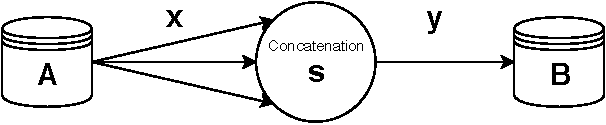
\includegraphics[width=0.48\textwidth]{Chapters/DeliveryGuarantees/pics/concat.pdf}
  \caption{Strings concatenation physical graph}
  \label{concat}
\end{figure}

\begin{table}[htbp]
\begin {center}
\caption{String concatenation data flow}   \tabcolsep2pt
\begin{tabular}{c|l|c|c|c|c|c|c}      
wall\\ time & $\tau$& $a\in A$  &$x\in W$& $s\in W$ & $y\in W$ & $b \in B$ & step  \\
\hline
1   &   1   &   a   &   a           &           &       &           &   input \\
1   &   2   &   c   &   a,c         &           &       &           &   input \\
1   &   3   &       &    c          &   [a]     &    a  &           &   transform \\
1   &   4   &       &   c           &   [a]     &       &   a       &   output \\
1   &   5   &       &               &   [a,c]   &   ac  &           &   transform \\
1   &   6   &       &               &   [a,c]   &       &   ac       &   output \\
1   &   7   &       &               &   [a,c]   &       &   [a,c]   &   snapshot \\
2   &   8   &   b    &   b          &   [a,c]   &       &           &   input \\
2   &   9   &   d    &   b,d        &   [a,c]   &       &           &   input \\
2   &   10   &       &   b          &   [c,d]   &  cd   &           &   transform \\
2   &   11   &       &   b          &   [c,d]   &       &      cd     &   output \\
2   &   12   &       &              &   [d,b]    &  db   &           &   transform \\
2   &   13   &       &              &   {\bf [d,b]}    &       &      {\bf db}     &   output \\
\arrayrulecolor{red}\hline
3   &   14   &       &               &   [a,c]         &       &           &   recovery \\
3   &   14   &   b   &   b           &   [a,c]         &       &           &   \\
3   &   14   &   d   &   b,d         &   [a,c]         &       &           &   \\
3   &   14   &       &   b           &   [c,d]         &       &           &   \\
3   &   14   &       &   b           &   [c,d]         &       &           &   \\
3   &   14   &       &               &   [d,b]         &       &           &    \\
3   &   14   &       &               &   {\bf [d,b]}   &       &           &    \\
\arrayrulecolor{red}\hline
4   &   15   &  e    &   e           &   [d,b]   &      &           &   input \\
4   &   16   &       &              &   [b,e]   &   be    &          &   transform \\
4   &   17   &       &              &   [b,e]   &       &   {\bf be}       &   output \\
\end{tabular}
\label{concat_example}
\end {center}
\end{table}

\subsection{Model analysis}

In a classical model proposed by Chandy and Lamport~\cite{Chandy:1985:DSD:214451.214456}, a distributed system is represented as a graph of processes, which can be connected via channels. Each process can own a modifiable internal state, generate {\em events} and send them to other processes through the channels. {\em Global system state} in this model contains processes states and channel states, e.g., elements, which are in-flight at the moment. Distributed asynchronous processing is simulated using permutations of events.

The proposed model is a variation of a classical Chandy-Lamport distributed system model with the following properties and modifications:

\begin{itemize}
    \item Our notion of a streaming system does not provide a concept of {\em operations state} because, as it is shown in~\cite{we2018adbis}, states can be considered as common data items. In this case, a state element is presented in a system until it is transformed into a new state together with new elements. This model allows a binary relation $D$ to capture computations within a graph of processes that is a physical streaming execution graph in our case. Hence, the working set $W_\tau$ is a global state with only channel states in terms of Chandy-Lamport.
    \item Input and output elements $a_\tau$ and $b_\tau$ are special events. This way, {\em storage} and {\em computations} are distinguished. We assume that output elements $B_\tau$ are all data that leaves a system including so-called {\em state snapshots} which are typically used for recovery~\cite{Carbone:2017:SMA:3137765.3137777}. Because of this, we state that $X \subseteq W_\tau \cup B_\tau$ in the transform transition of the working set. In most state-of-the-art stream processing systems, the end-user is external to the system, i.e., a user can observe input and output elements, but not the working set.
    \item Distributed asynchronous computations are modeled through the random choice of an operation that is executed next. In the proposed model, instead of using permutations of data flow elements that fixate an execution route, we suppose that the next transition of the working set is a random variable. The distribution of this variable depends on system architecture. 
\end{itemize}

\subsection{Consistent input and output}

The parallel asynchronous nature of distributed stream processing allows us to handle only a {\em probability} of an output element because it can be different from run to run due to element reorderings.

\begin{definition}{Probability of output element}
$P(b_{\tau+1}|A_{\tau}, B_\tau, F)$ is a probability to observe output element $b_{\tau+1}$ considering all previous input and output elements, and recovery function.
\end{definition}

The problem here is that it is hard to define the correct output, because it may significantly vary. Inconsistencies may arise only in case of failure and incorrect recovery. Let us introduce a {\em reference} recovery function that allows us to denote results which are possible to reach without failures.

\begin{definition}{Reference}
$F^{*}$ is a recovery function that restores exactly the same working set as before the failure, $\forall \tau \in \mathbb{N}, F^{*}(A_\tau,B_\tau)=W_\tau$.
\end{definition}

\begin{definition}{Probability of output element with a reference recovery function}
$P(b_{\tau+1}|A_{\tau}, B_\tau, F^{*})$ is a probability to observe output element $b_{\tau+1}$ considering all previous input and output elements, and a reference recovery function.
\end{definition}

Using the notion of a reference recovery function, one can define the correct output. 

\begin{definition}{Output element $b_{\tau+1}$ is consistent}
with all previous input and output elements $A_\tau$ and $B_\tau$ if the probability to observe it is non-zero in a system with reference recovery: $P(b_{\tau+1} \mid A_\tau,B_\tau,F^{*})>0$.
\end{definition}

The reference recovery function allows us to express the notion of correct execution in terms of correspondence between input and output elements. In most real cases, input and output elements are the only data that can be observed by the end-user. In real distributed stream processing systems, failures and recoveries can corrupt the output, despite the fact, that in terms of a simple definition of delivery guarantees, all elements are processed exactly-once. 

The problem here is that elements can be concatenated in a different order on recovery. Let us demonstrate it by the already mentioned example demonstrated in Figure~\ref{concat} and Table~\ref{concat_example}. During recovery system may reach concatenation state $s=[b,d]$ at $\tau=15$ rather than $s=[d,b]$ due to asynchronous input. In this case, output at $\tau=17$ becomes {\em de} instead of {\em be}. However, {\em de} is inconsistent with the previous output, because element with prefix {\em d} has already been released at $\tau=13$. It is important to note that all input elements within the example are applied to concatenation state {\em  exactly-once}. This simple example demonstrates that informal definition of exactly-once does not guarantee the consistency of output elements.

\subsection{Delivery guarantees}

As we demonstrate further, state-of-the-art stream processing systems prevent inconsistencies illustrated in the example above. However, the informal definition of exactly-once is insufficient to describe the level of data consistency that is provided. Here we introduce regular definitions of delivery guarantees which take this issue into account. 

\begin{definition}{System provides for exactly-once}
if it is possible to obtain each output element $b_{\tau+1}$ in a system with a reference recovery fucntion, i.e.,\\ 
$\forall{\tau \in \mathbb{N}}, b_{\tau+1}\in 2^{\Gamma}: P(b_{\tau+1}|A_{\tau},B_\tau,F)>0 \Rightarrow \\ P(b_{\tau+1}|A_{\tau},B_\tau,F^{*})>0$.
\end{definition}

\begin{definition}{System provides for at-most-once}
if \\
$\exists{A^{0}_{\tau}\subseteq{A_{\tau}}}$ such that \\
$\forall{\tau \in \mathbb{N},{b_{\tau+1}\in 2^{\Gamma}}}: P(b_{\tau+1}|A_{\tau},B_\tau,F)>0 \Rightarrow \\ P(b_{\tau+1}|A^{0}_{\tau},B_\tau,F^{*})>0$.
\end{definition}

\begin{definition}{System provides for at-least-once}
if \\
$\exists{A^{*}_{\tau}\subseteq{2^{A_{\tau}}}}$ such that \\
$\forall{\tau \in \mathbb{N}, {b_{\tau+1} \in 2^{\Gamma}}}: P(b_{\tau+1}|A_{\tau},B_\tau,F)>0 \Rightarrow \\ P(b_{\tau+1}|A^{*}_{\tau},B_\tau,F^{*})>0$.
\end{definition}

Exactly-once states that observed results cannot be distinguished from one of the possible results produced by a system with a reference recovery function. It means that even if data flow contains races and some elements do not commute, output consistency will be preserved. Looking back to the example illustrated in Table~\ref{concat_example}, our formal definition of exactly-once ensures that after recovery system reaches state $[d,b]$, not $[b,d]$, because this state has already influenced output elements.

At-most-once and at-least-once guarantees are the relaxations of exactly-once. The results within these guarantees can be obtained without failures, but with the modification of the input. At-least-once can be reproduced if the input contains duplicated items. At-most-once can be achieved with a reference recovery if some input elements are missed. It is important to note, that regarding at-most-once guarantee we require an input element to be processed atomically with all its derivatives or not processed at all. To the best of our knowledge, none of the stream processing engines supports at-most-once guarantee, so we cannot verify the relevancy of this assumption. It is accessible to provide at-most-once by producing no output at all, but if the output is presented, at-most-once enforcement becomes much more difficult.  

In our formal model, the relaxations of exactly-once are defined without diving into recovery mechanisms. Instead, they are described through possible input channel flaws in a system with a reference recovery. This trick allows us to represent invisible system details in terms clear for an external user.

